\section{Introduction}

In this document we discuss studies to define and understand triggers to be used to perform
searches with Photon(s), Jet(s) and MET in the final state.  Supersymmetry with General Gauge Mediated 
Symmetry Breaking (GGMSB) (ref) is used as the theoretical framework on which to base these searches.
Depending on the parameters defining the model, SUSY with GGMSB can span a wide range of experimental
signatures.  

At the LHC any SUSY particles produced are expected to have occurred via strong interactions, which would
imply production of ligher squarks and gluinos.  Decay of these particles could potentially result
in large amounts of jet activity in the event.  If within GGMSB one takes the gravitino as the lightest 
SUSY particle (LSP), and the lightest neutralino to be the next-to-lightest particle (NLSP), decay
of the squarks and gluinos may proceed through production of neutralinos and gluinos.  Neutralinos 
themselves can decay into a photon and gravitino, where the gravitino exits the detector undetected.
The final state detected would be some number of prompt photons from neutralino decay, jets from squark
and gluino decay products, and missing energy.  The "jettyness", number of photons and MET in the 
final state would depend on the exact (and unknown) parameters fed into the model, which implies a 
need for flexibility in the final states used to search for or constrain such a model.

For the 2010 collider run the SUSY GGMSB search (ref) was pursued via an analysis of diphoton events
with jets and MET.  A series of triggers were used as luminosity increased several orders of magnitude 
to $2\times10^{32} cm^2/s$.  Figure \ref{fig:photon22rate} shows the rate of the 
HLT\_Photon22\_SC22HE\_L1R trigger, used to select events for the analysis by the end of the run.  
Plotted are the trigger rates for each lumisection in three runs towards the end of November,
versus the instantaneous luminosity of those lumisections.  As the luminosity reached $2\times10^{32} cm^2/s$
the trigger rate approached 15 Hz.  

 \begin{figure}[!ht]
  \centering
 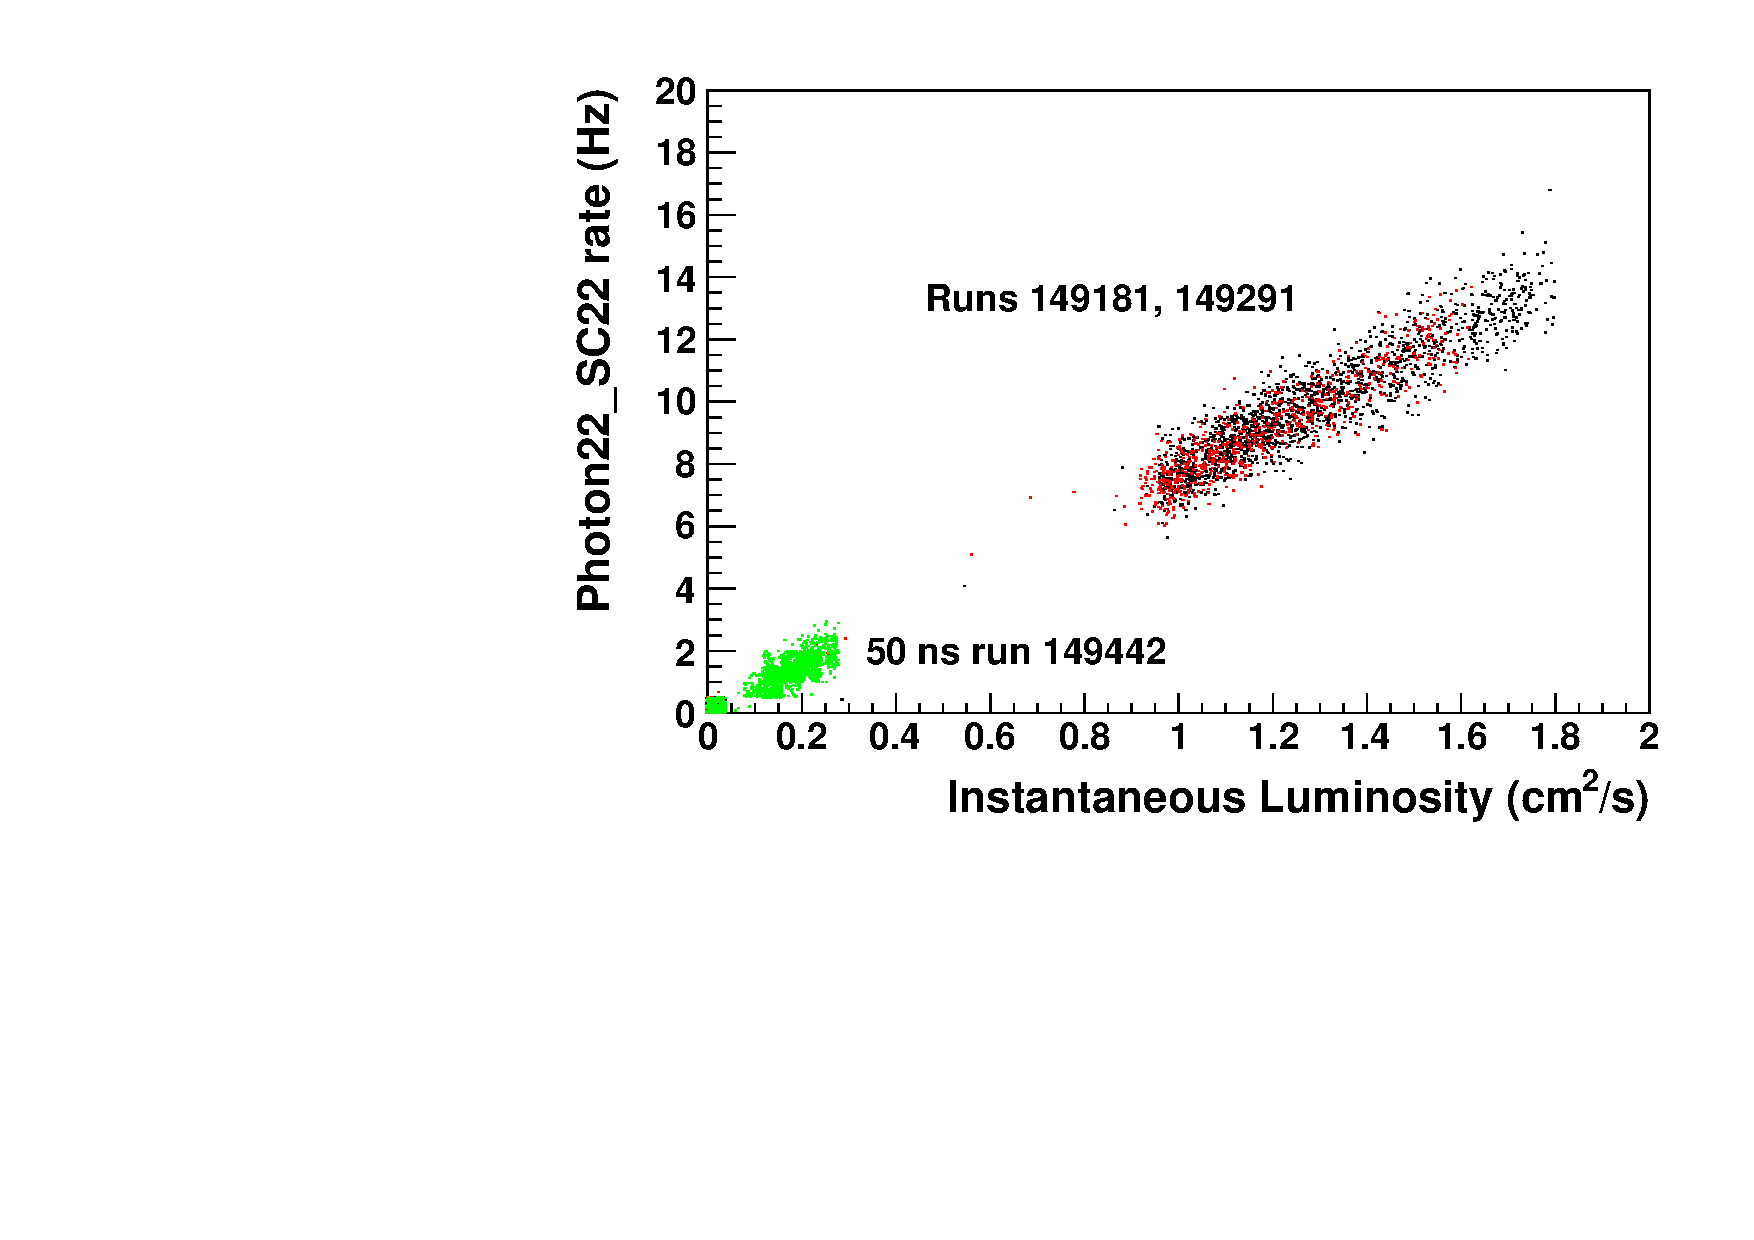
\includegraphics[width=0.85\textwidth]{figures/photon22rates.pdf}
\caption{Scatter plot of HLT\_Photon22\_SC22HE\_L1R trigger rates versus instantaneous luminosity for runs 
149181 (black), 149291 (red) and 149442 (green).  In run149442 the LHC ran with a 50 ns bunch spacing.}
\label{fig:photon22rate}
\end{figure}

Shortly after startup in the upcoming 2011 run, instantaneous luminosity is expected to reach 
$5\times10^{32} cm^2/s$, and in short order top $10^{33} cm^2/s$
later in the spring.  Rates from the triggers relied on last year will be too high to be used unprescaled in 2011. 

Because of the wide variation available in final states produced within GGMSB it is prudent to try to 
cast "as wide a net" as possible to avail detection, while living within rate constraints resulting from 
high luminosity and pile-up.  GGMSB as described above predicts events which in addition to one or more photons 
in the final state, have missing energy due to the exiting gravitino(s) as well
as considerable jet activity.  As the jets in the event can be plentiful but soft $H_T$, the scalar sum
of jet transverse momenta should be a good quantity to trigger by.  With the expected large number of simultaneous
interactions in each event, missing $H_T$, the vector sum of jet transverse momenta above a threshold, is 
expected to be useful for detecting missing energy while being less sensitive to pile-up.  We therefore
concentrate on defining triggers based on photon transverse energy, the $H_T$ of an event, and its $MH_T$.

